\documentclass[12pt]{article}

\usepackage{fancyhdr} % Required for custom headers
\usepackage{lastpage} % Required to determine the last page for the footer
\usepackage{extramarks} % Required for headers and footers
\usepackage[usenames,dvipsnames]{color} % Required for custom colors
\usepackage{graphicx} % Required to insert images
\usepackage{listings} % Required for insertion of code
\usepackage{courier} % Required for the courier font
\usepackage{lipsum} % Used for inserting dummy 'Lorem ipsum' text into the template
\usepackage{amsmath}
\usepackage{caption}
\usepackage{multirow}
\usepackage[dvipsnames]{xcolor}

\newcommand*{\addheight}[2][.5ex]{%
	\raisebox{0pt}[\dimexpr\height+(#1)\relax]{#2}%
}
% Margins
\topmargin=-0.45in
\evensidemargin=0in
\oddsidemargin=0in
\textwidth=6.5in
\textheight=9.0in
\headsep=0.25in
\headheight=15.0pt


\linespread{1.1} % Line spacing

% Set up the header and footer
\pagestyle{fancy}
\lhead{\hmwkAuthorName} % Top left header
\chead{\hmwkClass: \hmwkTitle} % Top center head
\cfoot{} % Bottom center footer
\rfoot{Page\ \thepage\ of\ \protect\pageref{LastPage}} % Bottom right footer
\renewcommand\headrulewidth{0.4pt} % Size of the header rule
\renewcommand\footrulewidth{0.4pt} % Size of the footer rule

\setlength\parindent{0pt} % Removes all indentation from paragraphs

%----------------------------------------------------------------------------------------
%	DOCUMENT STRUCTURE COMMANDS
%	Skip this unless you know what you're doing
%----------------------------------------------------------------------------------------

% Header and footer for when a page split occurs within a problem environment
\newcommand{\enterProblemHeader}[1]{
	\nobreak\extramarks{#1}{#1 continued on next page\ldots}\nobreak
	\nobreak\extramarks{#1 (continued)}{#1 continued on next page\ldots}\nobreak
}

% Header and footer for when a page split occurs between problem environments
\newcommand{\exitProblemHeader}[1]{
	\nobreak\extramarks{#1 (continued)}{#1 continued on next page\ldots}\nobreak
	\nobreak\extramarks{#1}{}\nobreak
}

\setcounter{secnumdepth}{0} % Removes default section numbers
\newcounter{homeworkProblemCounter} % Creates a counter to keep track of the number of problems

\newcommand{\homeworkProblemName}{}
\newenvironment{homeworkProblem}[1][Problem \arabic{homeworkProblemCounter}]{ % Makes a new environment called homeworkProblem which takes 1 argument (custom name) but the default is "Problem #"
	\stepcounter{homeworkProblemCounter} % Increase counter for number of problems
	\renewcommand{\homeworkProblemName}{#1} % Assign \homeworkProblemName the name of the problem
	\section{\homeworkProblemName} % Make a section in the document with the custom problem count
	\enterProblemHeader{\homeworkProblemName} % Header and footer within the environment
}{
	\exitProblemHeader{\homeworkProblemName} % Header and footer after the environment
}

\newcommand{\problemAnswer}[1]{ % Defines the problem answer command with the content as the only argument
	\noindent\framebox[\columnwidth][c]{\begin{minipage}{0.98\columnwidth}#1\end{minipage}} % Makes the box around the problem answer and puts the content inside
}

\newcommand{\homeworkSectionName}{}
\newenvironment{homeworkSection}[1]{ % New environment for sections within homework problems, takes 1 argument - the name of the section
	\renewcommand{\homeworkSectionName}{#1} % Assign \homeworkSectionName to the name of the section from the environment argument
	\subsection{\homeworkSectionName} % Make a subsection with the custom name of the subsection
	\enterProblemHeader{\homeworkProblemName\ [\homeworkSectionName]} % Header and footer within the environment
}{
	\enterProblemHeader{\homeworkProblemName} % Header and footer after the environment
}

%----------------------------------------------------------------------------------------
%	NAME AND CLASS SECTION
%----------------------------------------------------------------------------------------

\newcommand{\hmwkTitle}{Assignment\ \#1} % Assignment title
\newcommand{\hmwkClass}{Practical Data Science} % Course/class
\newcommand{\hmwkAuthorName}{Shikhar Vashishth} % Your name
\newcommand{\hmwkAuthorID}{M.Tech CSA - 13374} % Your ID

%----------------------------------------------------------------------------------------
%	TITLE PAGE
%----------------------------------------------------------------------------------------

\title{
	\vspace{2in}
	\textmd{\textbf{\hmwkClass}}\\ 
	\textmd{\textbf{\hmwkTitle}}\\
	\vspace{3in}
}

\author{\textbf{\hmwkAuthorName} \\ {\small \hmwkAuthorID}}
\date{} % Insert date here if you want it to appear below your name

%----------------------------------------------------------------------------------------

\begin{document}
	
\maketitle
\newpage


\clearpage
\begin{homeworkProblem}
\subsection{Part (a):}

\begin{figure}[ht]
	\centering
	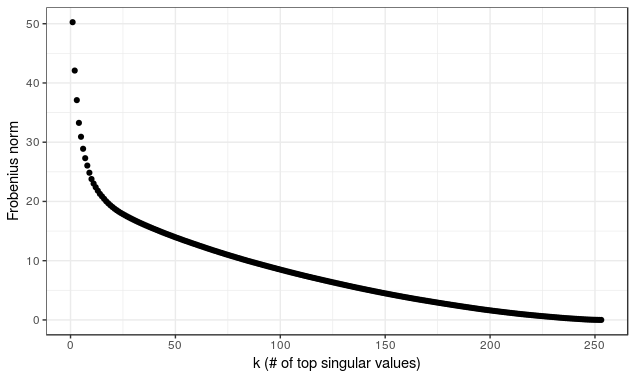
\includegraphics[width=14cm]{./q1/svd.png}
	\caption{Plot of $||X-Z_k||_F$ vs k}
\end{figure}

\begin{figure}[h]
	\centering
	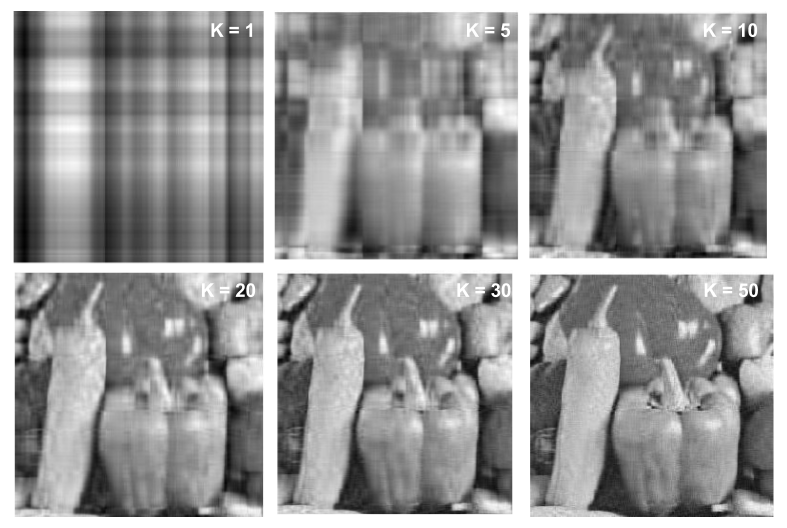
\includegraphics[scale=.35]{./svd/main.png}
	\caption{Approximation of image with different number of top singular values}
\end{figure}


\paragraph{Justification:}
We can see clearly from the above plot and images that as we increase the values of k, the number of top singular values used for approximating the original image, the quality of image improves. The plot was generated using R (ggplot2 library). 

\clearpage

\subsection{Part (b):}
\textbf{Time Comparison:}
\begin{center}
	\begin{tabular}{ |c||c|c|c|c|c|c|  }
		\hline
		Data density \% & CPU Time(sec) - SVT (250 iters) & CPU Time(sec) ISVD \\ 	\hline \hline
		10 & 4.1304 & 3.0991 \\ \hline
		20 & 3.9124 & 3.2581 \\ \hline
		30 & 4.2556 & 3.0166 \\ \hline
		40 & 4.1700 & 3.1476 \\ \hline
		50 & 4.1667 & 3.2274 \\ \hline
		60 & 4.1765 & 3.2299 \\ \hline
		70 & 4.3894 & 3.1999 \\ \hline
		80 & 4.1236 & 3.3031 \\ \hline
		90 & 4.1697 & 3.0940 \\ \hline		
		\hline
	\end{tabular}
\end{center}

\textbf{Frobenius norm comparison} ($||X_{org}-X_{apprx}||_F$):
\begin{figure}[h]
	\centering
	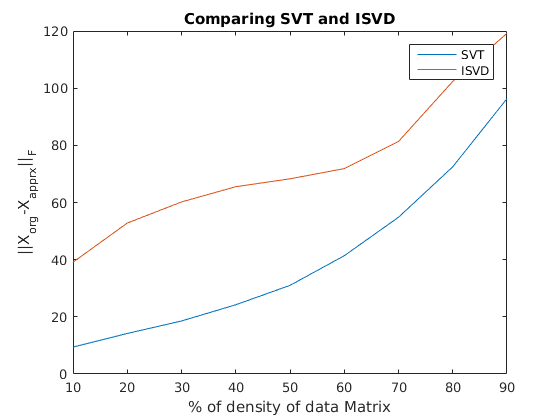
\includegraphics[scale=1]{./q1/comp_svt_isvd.png}
	\caption{Comparing SVT and ISVD algorithms}
\end{figure}

\clearpage

\textbf{Visual Comparison:}

\begin{figure}[h]
	\centering
	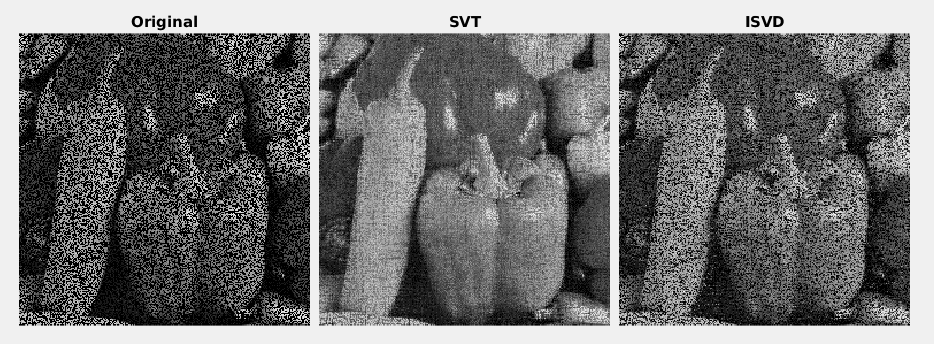
\includegraphics[scale=.5]{./q1/1.png}
	\caption{Comparing SVT and ISVD result for data density 50 \%}
\end{figure}
\begin{figure}[h]
	\centering
	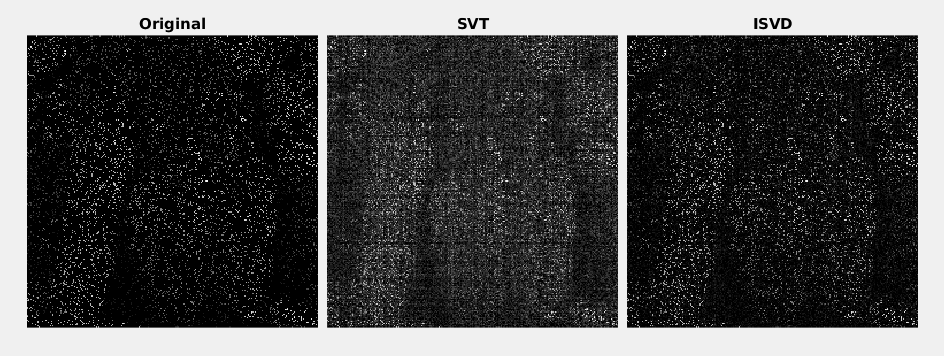
\includegraphics[scale=.5]{./q1/2.png}
		\caption{Comparing SVT and ISVD result for data density 10 \%}
\end{figure}

\paragraph{Justification:}
From the given results we can conclude that although Singular value thresholding algorithm takes more time compared to ISVD algorithm but the performance of SVT is much better than ISVD. The frobenius norm of difference ($||X_{org}-X_{apprx}||_F$) clearly reveals this fact. The visual results also support this observation from the figure 4 and 5 we can see that how SVT algorithm's results are much superior than that of ISVD algorithm's results.
\end{homeworkProblem}

\clearpage
\begin{homeworkProblem}
\subsubsection{Formulation (A)}
\begin{equation*}
\begin{aligned}
& \underset{W,H}{\text{minimize}}
& & \frac{1}{2}||X-WH||_F^2 + \frac{\tau}{2}(||W||_F^2 + ||H||_F^2)\\
& \text{subject to}	
& & W, H \ge 0\\
\end{aligned}
\end{equation*}

\subsubsection{Formulation (B)}
\begin{equation*}
\begin{aligned}
& \underset{W,H}{\text{minimize}}
& & \frac{1}{2}||X-WH||_F^2 + \tau(||W||_1 + ||H||_1)\\
& \text{subject to}
& & W, H \ge 0\\
\end{aligned}
\end{equation*}

\subsubsection{Formulation (C)}
\begin{equation*}
\begin{aligned}
& \underset{W,H}{\text{minimize}}
& & \sum_{i,j} \left(X_{ij} \log{\frac{X_{ij}}{(WH)_{ij}}} - X_{ij} + (WH)_{ij} \right) + \frac{\tau}{2}(||W||_F^2 + ||H||_F^2)\\
& \text{subject to}
& & W, H \ge 0\\
\end{aligned}
\end{equation*}


\subsection{Results:}
\begin{center}
	\begin{tabular}{ |c||c|c|c|c|c|c|  }
	\hline
	 & $\tau$ & Iters & CPU Time(sec) & Spar. \% of W & Spar. \% of H & $||X - WH||_F^2$\\
	\hline \hline
	\multirow{3}{4.5em}{Form (A) Random} 	& 1000 	& 100 & 1.427 & -     & -     & - \\
											& 1 	& 100 & 0.708 & 38.80 & 17.11 & 45.90 \\
											& .001 	& 100 & 0.785 & 40.84 & 22.70 & 45.78 \\ \hline
											
	\multirow{3}{5em}{Form (A) NNDSVD} 		& 1000 	& 100 & 1.700 & - & -  & - \\
											& 1 	& 100 & 0.907 & 37.14 & 15.18 & 45.84 \\
											& .001 	& 100 & 0.828 & 41.74 & 24.72 & 45.78 \\ \hline
											
	\multirow{3}{5em}{Form (B) Random} 		& 1000 	& 100 & 0.781 & - & - & - \\
											& 1 	& 100 & 0.797 & - & - & - \\
											& .001 	& 100 & 0.816 & 43.24 & 29.70 & 45.83 \\ \hline
	
	\multirow{3}{4.5em}{Form (B) NNDSVD} 	& 1000 	& 100 & 0.933 & - & - & - \\
											& 1 	& 100 & 0.840 & - & - & - \\
											& .001 	& 100 & 0.875 & 44.16 & 26.32 & 45.78 \\ \hline
											
	\multirow{3}{4.5em}{Form (C) Random} 	& 1000 	& 50  & 791.28 & 54.85 & 42.55 & 46.05 \\
											& 1 	& 50  & 790.55 & 55.77 & 42.47 & 46.02 \\
											& .001 	& 50  & 800.31 & 53.43 & 29.14 & 46.51 \\ \hline
											
	\multirow{3}{5em}{Form (C) NNDSVD} 		& 1000 	& 50  & 854.63 & 55.18 & 34.75 & 46.50 \\
											& 1 	& 50  & 802.68 & 54.35 & 53.19 & 45.94 \\
											& .001 	& 50  & 790.88 & 54.32 & 53.21 & 45.94 \\ \hline
	
	\hline
	\end{tabular}
\end{center}

Sparsity is calculated as:
$$ Sparsity = \frac{\text{\# of Zero entries}(< .000001)}{\text{Total entries}}$$

\subsubsection{Formulation (A): Random Intialization}

$\tau = 1000 \rightarrow$  No meaningful result \\
$\tau = 1 \rightarrow$ 

\begin{center}
	\begin{tabular}{||c c c c c||} 
		\hline
		$W_1$ & $W_2$ & $W_3$ & $W_4$ & $W_5$\\ [0.5ex] 
		\hline\hline
		growth &      mobile &        yukos &      mr &            film \\ \hline   
		economy &     people &        said &       labour &        best \\ \hline   
		economic &    music &         russian &    election &      england \\ \hline
		sales &       said &          oil &        blair &         game \\ \hline   
		year &        digital &       court &      brown &         win \\ \hline    
		said &        phone &         company &    party &         said \\ \hline   
		2004 &        technology &    gazprom &    said &          won \\ \hline    
		prices &      users &         mr &         howard &        year \\ \hline   
		bank &        broadband &     firm &       government &    wales \\ \hline  
		rate &        phones &        russia &     minister &      play \\ \hline  \hline
		\textbf{business} & \textbf{tech} & \textbf{business} & \textbf{politics} & \textbf{entertainment} \\ \hline
	\end{tabular}
\end{center}

$\tau = 0.001 \rightarrow$
\begin{center}
	\begin{tabular}{||c c c c c||} 
		\hline
		$W_1$ & $W_2$ & $W_3$ & $W_4$ & $W_5$\\ [0.5ex] 
		\hline\hline
	    growth &      mr &            mobile &        film &        england \\ \hline
	economy &     labour &        people &        best &        game \\ \hline   
	said &        blair &         music &         awards &      win \\ \hline    
	bank &        election &      said &          award &       wales \\ \hline  
	sales &       brown &         digital &       actor &       ireland \\ \hline
	year &        party &         technology &    oscar &       cup \\ \hline    
	economic &    said &          phone &         actress &     said \\ \hline   
	oil &         government &    users &         festival &    team \\ \hline   
	prices &      howard &        broadband &     won &         play \\ \hline   
	2004 &        minister &      software &      films &       players \\ \hline \hline  
	\textbf{business} & \textbf{politics} & \textbf{tech} & \textbf{entertainment} & \textbf{sports} \\ \hline
	\end{tabular}
\end{center}
\paragraph{Justification}
We can easily see that how the algorithm varies with different values of $\tau$, when using $\tau = 1000$ the algorithm didn't give any meaningful results and even when $\tau$ was made 1000 the topics predicted were not complete (sports category missing). But with $\tau = .001$ the algorithm gave the desired results.
\clearpage
\subsubsection{Formulation (A): NNDSVD Intialization}

$\tau = 1000 \rightarrow$  No meaningful result \\
$\tau = 1 \rightarrow$ 

\begin{center}
	\begin{tabular}{||c c c c c||} 
		\hline
		$W_1$ & $W_2$ & $W_3$ & $W_4$ & $W_5$\\ [0.5ex] 
		\hline\hline
		    mr &            england &    growth &      film &        mobile \\ \hline    
		labour &        game &       economy &     best &        people \\ \hline    
		blair &         win &        said &        awards &      music \\ \hline     
		election &      wales &      year &        award &       said \\ \hline      
		brown &         ireland &    bank &        actor &       digital \\ \hline   
		party &         said &       sales &       oscar &       technology \\ \hline
		said &          cup &        economic &    actress &     phone \\ \hline     
		government &    team &       oil &         festival &    users \\ \hline     
		howard &        play &       2004 &        won &         broadband \\ \hline 
		minister &      players &    prices &      films &       software \\ \hline  \hline
		\textbf{politics} & \textbf{sports} & \textbf{business} & \textbf{entertainment} & \textbf{tech} \\ \hline
	\end{tabular}
\end{center}

$\tau = 0.001 \rightarrow$
\begin{center}
	\begin{tabular}{||c c c c c||} 
		\hline
		$W_1$ & $W_2$ & $W_3$ & $W_4$ & $W_5$\\ [0.5ex] 
		\hline\hline
		mr &            england &    growth &      film &        mobile \\ \hline    
		labour &        game &       economy &     best &        people \\ \hline    
		blair &         win &        said &        awards &      music \\ \hline     
		election &      wales &      bank &        award &       said \\ \hline      
		brown &         ireland &    year &        actor &       digital \\ \hline   
		party &         cup &        sales &       oscar &       technology \\ \hline
		said &          said &       economic &    actress &     phone \\ \hline     
		government &    team &       oil &         festival &    users \\ \hline     
		howard &        play &       prices &      films &       broadband \\ \hline 
		minister &      players &    2004 &        won &         software \\ \hline  \hline
		\textbf{politics} & \textbf{sports} & \textbf{business} & \textbf{entertainment} & \textbf{tech} \\ \hline 
	\end{tabular}
\end{center}
\paragraph{Justification}
The NNDSVD intialization greatly improved the performance of the algorithm, we can see clearly that although with random initialization and $\tau = 1$ the algorithm didn't give correct results but with NNDSVD intialization it gave the desired results for both values of $\tau$ (1 and .001) and there is improvement in frobenius norm as well.

\clearpage
\subsubsection{Formulation (B): Random Intialization}

$\tau = 1000 \rightarrow$  No meaningful result \\
$\tau = 1 \rightarrow$ No meaningful result \\
$\tau = 0.001 \rightarrow$
\begin{center}
	\begin{tabular}{||c c c c c||} 
		\hline
		$W_1$ & $W_2$ & $W_3$ & $W_4$ & $W_5$\\ [0.5ex] 
		\hline\hline
		mobile &        film &       growth &      mr &            yukos \\ \hline  
		people &        best &       economy &     labour &        said \\ \hline   
		music &         england &    economic &    election &      russian \\ \hline
		digital &       game &       sales &       blair &         court \\ \hline  
		phone &         win &        year &        brown &         company \\ \hline
		technology &    said &       said &        party &         oil \\ \hline    
		said &          won &        prices &      said &          gazprom \\ \hline
		broadband &     year &       2004 &        howard &        law \\ \hline    
		users &         wales &      bank &        government &    firm \\ \hline   
		phones &        play &       rate &        minister &      mr \\ \hline        \hline
		\textbf{tech} & \textbf{sports} & \textbf{business} & \textbf{politics} & \textbf{business} \\ \hline 
	\end{tabular}
\end{center}


\subsubsection{Formulation (B): NNDSVD Intialization}

$\tau = 1000 \rightarrow$  No meaningful result \\
$\tau = 1 \rightarrow$ No meaningful result \\
$\tau = 0.001 \rightarrow$
\begin{center}
	\begin{tabular}{||c c c c c||} 
		\hline
		$W_1$ & $W_2$ & $W_3$ & $W_4$ & $W_5$\\ [0.5ex] 
		\hline\hline
		mr &            england &    growth &      film &        mobile \\ \hline    
		labour &        game &       economy &     best &        people \\ \hline    
		blair &         win &        said &        awards &      music \\ \hline     
		election &      wales &      bank &        award &       said \\ \hline      
		brown &         ireland &    year &        actor &       digital \\ \hline   
		party &         cup &        sales &       oscar &       technology \\ \hline
		said &          said &       economic &    actress &     phone \\ \hline     
		government &    team &       oil &         festival &    users \\ \hline     
		howard &        play &       prices &      films &       broadband \\ \hline 
		minister &      players &    2004 &        won &         software \\ \hline   \hline
		\textbf{politics} & \textbf{sports} & \textbf{business} & \textbf{entertainment} & \textbf{tech} \\ \hline  
	\end{tabular}
\end{center}

\paragraph{Justification}
With formulation (B), the gradient descent approach didn't perform well with $\tau$ value as 1000 and 1, for both of them it gave meaningless results. But with $\tau$ value as .001 the algorithm gave the desired results. With NNDSVD intializaiton the frobenius norm value decreased. 

\clearpage
\subsubsection{Formulation (C): Random Intialization}

$\tau = 1000 \rightarrow$  
\begin{center}
	\begin{tabular}{||c c c c c||} 
		\hline
		$W_1$ & $W_2$ & $W_3$ & $W_4$ & $W_5$\\ [0.5ex] 
		\hline\hline
		    music &         england &    said &       film &      mr \\ \hline        
		said &          game &       growth &     best &      said \\ \hline      
		people &        team &       economy &    awards &    labour \\ \hline    
		users &         wales &      market &     award &     election \\ \hline  
		software &      ireland &    year &       won &       blair \\ \hline     
		games &         said &       bank &       said &      party \\ \hline     
		band &          players &    company &    actor &     government \\ \hline
		online &        injury &     sales &      year &      people \\ \hline    
		technology &    chelsea &    oil &        oscar &     brown \\ \hline     
		microsoft &     rugby &      china &      star &      minister \\ \hline   \hline
		\textbf{tech} & \textbf{sports} & \textbf{business} & \textbf{entertainment} & \textbf{politics} \\ \hline 
	\end{tabular}
\end{center}   
$\tau = 1 \rightarrow$ 

\begin{center}
	\begin{tabular}{||c c c c c||} 
		\hline
		$W_1$ & $W_2$ & $W_3$ & $W_4$ & $W_5$\\ [0.5ex] 
		\hline\hline
		    england &    mr &            mobile &        film &        said \\ \hline    
		game &       said &          people &        best &        growth \\ \hline  
		win &        government &    music &         awards &      sales \\ \hline   
		cup &        labour &        digital &       award &       economy \\ \hline 
		said &       election &      phone &         band &        year \\ \hline    
		club &       blair &         technology &    said &        2004 \\ \hline    
		match &      party &         said &          year &        bank \\ \hline    
		team &       brown &         games &         star &        prices \\ \hline  
		wales &      minister &      tv &            album &       market \\ \hline  
		injury &     tax &           broadband &     festival &    economic \\ \hline \hline
		\textbf{sports} & \textbf{politics} & \textbf{tech} & \textbf{entertainment} & \textbf{business} \\ \hline 
	\end{tabular}
\end{center}

$\tau = 0.001 \rightarrow$
\begin{center}
	\begin{tabular}{||c c c c c||} 
		\hline
		$W_1$ & $W_2$ & $W_3$ & $W_4$ & $W_5$\\ [0.5ex] 
		\hline\hline
		    said &          game &       mr &            film &      mobile \\ \hline    
		economy &       england &    said &          best &      people \\ \hline    
		growth &        win &        labour &        awards &    said \\ \hline      
		government &    said &       blair &         band &      technology \\ \hline
		mr &            cup &        party &         music &     music \\ \hline     
		year &          play &       election &      award &     digital \\ \hline   
		bank &          match &      government &    album &     users \\ \hline     
		economic &      team &       people &        said &      software \\ \hline  
		oil &           club &       howard &        star &      phone \\ \hline     
		market &        players &    minister &      actor &     net \\ \hline     	  \hline
		\textbf{business} & \textbf{sports} & \textbf{politics} & \textbf{entertainment} & \textbf{tech} \\ \hline 
	\end{tabular}
\end{center}


\subsubsection{Formulation (C): NNDSVD Intialization}

$\tau = 1000 \rightarrow$  No meaningful result \\
\begin{center}
	\begin{tabular}{||c c c c c||} 
		\hline
		$W_1$ & $W_2$ & $W_3$ & $W_4$ & $W_5$\\ [0.5ex] 
		\hline\hline
		    mr &            film &        said &       game &       people \\ \hline    
		said &          best &        growth &     england &    mobile \\ \hline    
		labour &        awards &      market &     win &        said \\ \hline      
		election &      award &       economy &    said &       technology \\ \hline
		blair &         music &       year &       cup &        users \\ \hline     
		government &    band &        company &    club &       software \\ \hline  
		party &         star &        bank &       match &      music \\ \hline     
		brown &         album &       sales &      team &       digital \\ \hline   
		minister &      festival &    oil &        injury &     computer \\ \hline  
		people &        actor &       firm &       players &    games \\ \hline   \hline
		\textbf{politics} & \textbf{entertainment} & \textbf{business} & \textbf{sports}  & \textbf{tech} \\ \hline 
	\end{tabular}
\end{center}   
$\tau = 1 \rightarrow$ 

\begin{center}
	\begin{tabular}{||c c c c c||} 
		\hline
		$W_1$ & $W_2$ & $W_3$ & $W_4$ & $W_5$\\ [0.5ex] 
		\hline\hline
		    mr &            film &      said &       england &    people \\ \hline    
		said &          best &      growth &     game &       mobile \\ \hline    
		labour &        awards &    economy &    win &        said \\ \hline      
		election &      award &     bank &       said &       technology \\ \hline
		blair &         music &     market &     club &       software \\ \hline  
		government &    band &      company &    cup &        users \\ \hline     
		party &         star &      year &       match &      digital \\ \hline   
		brown &         year &      sales &      team &       games \\ \hline     
		minister &      said &      oil &        injury &     phone \\ \hline     
		people &        album &     china &      players &    music \\ \hline     \hline
		\textbf{politics} & \textbf{entertainment} & \textbf{business} & \textbf{sports} & \textbf{tech} \\ \hline 
	\end{tabular}
\end{center}

$\tau = 0.001 \rightarrow$
\begin{center}
	\begin{tabular}{||c c c c c||} 
		\hline
		$W_1$ & $W_2$ & $W_3$ & $W_4$ & $W_5$\\ [0.5ex] 
		\hline\hline
		    mr &            film &      said &       england &    people \\ \hline    
		said &          best &      growth &     game &       mobile \\ \hline    
		labour &        awards &    economy &    win &        said \\ \hline      
		election &      award &     bank &       said &       technology \\ \hline
		blair &         music &     market &     club &       software \\ \hline  
		government &    band &      company &    cup &        users \\ \hline     
		party &         star &      year &       match &      digital \\ \hline   
		brown &         year &      sales &      team &       games \\ \hline     
		minister &      said &      oil &        injury &     phone \\ \hline     
		people &        album &     china &      players &    music \\ \hline    \hline
		\textbf{politcs} & \textbf{entertainment} & \textbf{business} & \textbf{sports} & \textbf{tech} \\ \hline 
	\end{tabular}
\end{center}

\paragraph{Justification}
With formulation (C), the algorithm gave the desired results for all values of $\tau$ (1000, 1, .001). The sparsity of computed $W$ and $H$ matrices was found to be much better as compared to the other two formulations. But in terms of computation time the algorithm is the worst.
\end{homeworkProblem}

\paragraph{Conclusion:}
From all the formulations the KL-divergence formulation is the most stable, as it gives the desired results for all values of $\tau$. Moreover, the sparsity of the generated W and H matrices also improves with this formulation. But the compuational time required for it is considerably higher as compared to other two formulations.
\end{document}